% Copyright 2021  Ed Bueler

\documentclass[xcolor={svgnames},
               hyperref={colorlinks,citecolor=DeepPink4,linkcolor=FireBrick,urlcolor=Maroon}]
               {beamer}

\mode<presentation>{
  \usetheme{Madrid}
  \usecolortheme{seagull}
  \setbeamercovered{transparent}
  \setbeamerfont{frametitle}{size=\large}
}

\setbeamercolor*{block title}{bg=red!10}
\setbeamercolor*{block body}{bg=red!5}

\usepackage[english]{babel}
\usepackage[latin1]{inputenc}
\usepackage{times}
\usepackage[T1]{fontenc}
% Or whatever. Note that the encoding and the font should match. If T1
% does not look nice, try deleting the line with the fontenc.

\usepackage{empheq,bm}
\usepackage{xspace}
\usepackage{fancyvrb}

\usepackage{tikz}
\usetikzlibrary{shapes,arrows.meta,decorations.markings,decorations.pathreplacing,fadings,positioning}

\usepackage[kw]{pseudo}
\pseudoset{left-margin=15mm,topsep=5mm,idfont=\texttt,st-left=,st-right=}


% If you wish to uncover everything in a step-wise fashion, uncomment
% the following command:
%\beamerdefaultoverlayspecification{<+->}

\newcommand{\ba}{\mathbf{a}}
\newcommand{\bb}{\mathbf{b}}
\newcommand{\bc}{\mathbf{c}}
\newcommand{\bbf}{\mathbf{f}}
\newcommand{\bg}{\mathbf{g}}
\newcommand{\bn}{\mathbf{n}}
\newcommand{\bq}{\mathbf{q}}
\newcommand{\br}{\mathbf{r}}
\newcommand{\bx}{\mathbf{x}}
\newcommand{\by}{\mathbf{y}}
\newcommand{\bv}{\mathbf{v}}
\newcommand{\bu}{\mathbf{u}}
\newcommand{\bw}{\mathbf{w}}

\newcommand{\bF}{\mathbf{F}}
\newcommand{\bG}{\mathbf{G}}
\newcommand{\bQ}{\mathbf{Q}}

\newcommand{\grad}{\nabla}
\newcommand{\Div}{\nabla\cdot}
\newcommand{\minmod}{\operatorname{minmod}}

\newcommand{\CC}{\mathbb{C}}
\newcommand{\RR}{\mathbb{R}}

\newcommand{\ddt}[1]{\ensuremath{\frac{\partial #1}{\partial t}}}
\newcommand{\ddx}[1]{\ensuremath{\frac{\partial #1}{\partial x}}}
\newcommand{\Matlab}{\textsc{Matlab}\xspace}
\newcommand{\Octave}{\textsc{Octave}\xspace}
\newcommand{\eps}{\epsilon}

\newcommand{\ip}[2]{\left<#1,#2\right>}

\newcommand{\xiphalf}{{x_{i+\frac{1}{2}}}}
\newcommand{\ximhalf}{{x_{i-\frac{1}{2}}}}
\newcommand{\Fiphalf}{{F_{i+\frac{1}{2}}}}
\newcommand{\Fimhalf}{{F_{i-\frac{1}{2}}}}
\newcommand{\Fiphalfn}{{F^n_{i+\frac{1}{2}}}}
\newcommand{\Fimhalfn}{{F^n_{i-\frac{1}{2}}}}

\newcommand{\trefcolumn}[1]{\begin{bmatrix} \phantom{x} \\ #1 \\ \phantom{x} \end{bmatrix}}
\newcommand{\trefmatrixtwo}[2]{\left[\begin{array}{c|c|c} & & \\ #1 & \dots & #2 \\ & & \end{array}\right]}
\newcommand{\trefmatrixthree}[3]{\left[\begin{array}{c|c|c|c} & & & \\ #1 & #2 & \dots & #3 \\ & & & \end{array}\right]}
\newcommand{\trefmatrixgroups}[4]{\left[\begin{array}{c|c|c|c|c|c} & & & & & \\ #1 & \dots & #2 & #3 & \dots & #4 \\ & & & & & \end{array}\right]}

\newcommand{\blocktwo}[4]{\left[\begin{array}{c|c} #1 & #2 \\ \hline #3 & #4 \end{array}\right]}

\newcommand{\bqed}{{\color{blue}\qed}}
\newcommand{\ds}{\displaystyle}

\newcommand\mynum[1]{{\renewcommand{\insertenumlabel}{#1}%
      \usebeamertemplate{enumerate item} \,}}


\title{Online optimization}

\subtitle{\emph{ML training algorithms minimize regret}}

\author{Ed Bueler}

\institute[UAF]{MATH 692 Mathematics for Machine Learning}

\date[Spring 2022]{17 March}

%\titlegraphic{\begin{picture}(0,0)
%    \put(0,180){\makebox(0,0)[rt]{\includegraphics[width=4cm]{figs/software.png}}}
%  \end{picture}
%}

%% to start section counter at 0 see
%% https://tex.stackexchange.com/questions/170222/change-the-numbering-in-beamers-table-of-content


\begin{document}
\beamertemplatenavigationsymbolsempty

\begin{frame}
  \maketitle
\end{frame}


\begin{frame}{Outline}
  \tableofcontents[hideallsubsections]
\end{frame}


\begin{frame}{but first, why am I talking about online optimization?}

\begin{itemize}
\item my motivations:
    \begin{itemize}
    \item[$-$] speaking as an optimization teacher: why is SGD so popular?
    \item[$-$] speaking as a numerical analyst: is my algorithm better than yours?
    \end{itemize}

\medskip
\item in trying to get my bearings, it was easy to stumble on:

\begin{center}
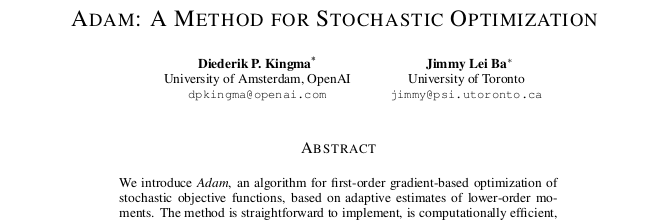
\includegraphics[width=0.7\textwidth]{figs/adam-paper.png}
\end{center}

\medskip
    \begin{itemize}
    \item[$-$] 100651 citations \dots for a conference paper
    \item[$-$] the Adam optimizer is the default for \href{https://www.tensorflow.org/tutorials/keras/classification}{tensorflow}, \href{https://pytorch.org/docs/stable/optim.html}{pytorch}, \dots
    \end{itemize}

\medskip
\item so, how do they show that Adam is good?
    \begin{itemize}
    \item[$-$] regret bound
    \item[$-$] see the remaining slides!
    \end{itemize}
\end{itemize}
\end{frame}


\section{online optimization framework}

\begin{frame}{training a neural net ($=$ recalling my earlier talk)}

\begin{itemize}
\item forward pass through an artificial neural net with $L$ layers:

\begin{columns}
\begin{column}{0.1\textwidth}
$x^{\{i\}}\to$ 
\end{column}
\begin{column}{0.4\textwidth}
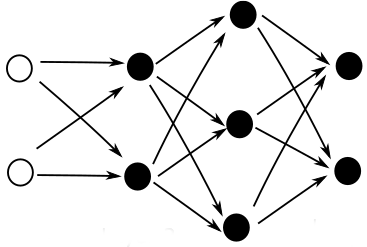
\includegraphics[height=30mm]{figs/cleannet.png}
\end{column}
\begin{column}{0.45\textwidth}
$\to a^{[L]}$ \hfill (supposed to be $y^{\{i\}}$)
\end{column}
\end{columns}

\item output activations are a function of input and parameters:
    $$a^{[L]} = a^{[L]}(x^{\{i\}}; p)$$
\item parameters $p$ collect weights and biases:
    $$p=\{W^{[2]},\dots,W^{[L]},b^{[2]},\dots,b^{[L]}\} \in \RR^n$$
\item cost of one labeled pair $(x^{\{i\}},y^{\{i\}})$:
    $$C^{\{i\}}(p) = \frac{1}{2} \left\|y^{\{i\}} - a^{[L]}(x^{\{i\}}; p)\right\|_2^2$$
\end{itemize}
\end{frame}


\begin{frame}{total cost objective versus online}

\begin{block}{training set total cost}
\textbf{original goal:}  minimize total cost over fixed training set
    $$C(p) = \frac{1}{N} \sum_{i=1}^N C^{\{i\}}(p)$$
\end{block}

\begin{block}{online training $=$ sequence of cost objectives}
assume infinite sequence of labeled pairs, equivalently of cost functionals:
    $$c_i(p) = C^{\{i\}}(p)$$
\textbf{method:} train neural net incrementally, a little for each $c_i$

\bigskip
\textbf{but what's the goal?}
\end{block}
\end{frame}


\begin{frame}{online training algorithms}

\begin{itemize}
\item $p_1$ is the initial iterate for the parameters
\item an \emph{online training algorithm} computes each new iterate $p_{j+1}$
    \begin{itemize}
    \item[$\circ$] generally, $p_{j+1}$ can be computed from all previous cost functionals $\{c_1,c_2,\dots,c_j\}$ and parameter iterates $\{p_1,p_2,\dots,p_j\}$
    \item[$\circ$] ``online'' $=$ we do not use future cost functionals
    \end{itemize}
\end{itemize}

\bigskip
\textbf{examples.}
\begin{itemize}
\item ``stochastic'' gradient descent with varying learning rates $\eta_j$:
   $$p_{j+1} = p_j - \eta_j \grad c_j(p_j)$$
\item Adam (\emph{more later})
\item Adaline, Adadelta, Adagrad, RMSprop, mini-batching, \dots
    \begin{itemize}
    \item[$\circ$] google search for buzzwords: \quad \texttt{tensorflow optimizers}
    \end{itemize}
\item online (quasi-)Newton methods; use/construct 2nd derivatives
\end{itemize}
\end{frame}


\section{regret}

\begin{frame}{regret of a training algorithm}

\begin{block}{\textbf{definition}}
the \emph{regret} of a training algorithm, at the $k$th step, is
    $$R_k = \sum_{j=1}^k c_j(p_j) - \min_p \sum_{j=1}^k c_j(p)$$
\end{block}

\begin{itemize}
\item regret is the difference between the algorithm result and the best possible result from a single parameter setting
\end{itemize}
\end{frame}


\begin{frame}{regret arose in game theory}

\begin{itemize}
\item treat the algorithm as a \emph{player} and the online stream of cost functionals $c_j$ as an \emph{adversary}
\item the player chooses $p_j$ \underline{before} knowing $c_j$
\end{itemize}

\begin{block}{online convex game (Abernathy et al 2008)}
\begin{pseudo*}
for $j = 1,2,\dots,k$: \\+
    \st{player chooses} $p_{j}$ \\
    \st{adversary chooses} $c_{j}$ \\-
end \\
\st{player suffers regret} \\+
    $\ds R_k = \sum_{j=1}^k c_j(p_j) - \min_p \sum_{j=1}^k c_j(p)$
\end{pseudo*}
\end{block}

\begin{itemize}
\item $R_k>0$: the player regrets not choosing $p = \operatorname{argmin} \sum_{j=1}^k c_j(p)$
\item but negative regret is possible!
\end{itemize}
\end{frame}


\begin{frame}{convex sets and functions}

\begin{itemize}
\item previous slide says ``convex''; we need the definition
\end{itemize}

\begin{block}{definition}
\begin{itemize}
\item a set $K \subset \RR^n$ is \emph{convex} if for all $x,y \in K$ and $0 \le t \le 1$,
  $$t\, x + (1-t) y \in K$$

    \begin{itemize}
    \item[$\circ$] the line segment from $x$ to $y$ is inside $K$
    \end{itemize}
\item a function $f:K \to \RR$ is \emph{convex} if for all $x,y \in K$ and $0 \le t \le 1$,
  $$t\, f(x) + (1-t) f(y) \ge f(t\, x + (1-t) y)$$
\end{itemize}
\end{block}

\begin{itemize}
\item for $f:K\to \RR$ to be convex, note $K$ must be convex
\item convex = concave \emph{up}
\end{itemize}
\end{frame}


\begin{frame}{convex optimization}

\begin{block}{definition}
given a convex set $K \subset \RR^n$ and a convex function $f:K\to \RR$, we say that the problem
    $$\min_{p \in K} f(p)$$
is a \emph{convex optimization problem}
\end{block}

\begin{itemize}
\item SVM is convex optimization, with nontrivial $K$
\item for an ANN, when is $C^{\{i\}}(p) = \frac{1}{2} \left\|y^{\{i\}} - a^{[L]}(x^{\{i\}}; p)\right\|_2^2$ a convex function on $K = \RR^n$?
\end{itemize}
\end{frame}


\begin{frame}{online convex optimization}

\begin{block}{definition}
\emph{online convex optimization}:  fix a convex set $K\subset \RR^n$, assume a sequence of convex functions $c_j:K\to \RR$, and seek to solve
    $$\min_{p_j \in K} c_j(p_j) \quad \text{or} \quad \min_{p \in K} \sum_{j=1}^k c_j(p)$$
\end{block}

\begin{itemize}
\item online convex optimization = online convex programming
\end{itemize}
\end{frame}


\begin{frame}{regarding regret}

\begin{itemize}
\item Zinkevich (2003): \emph{We cannot hope to choose a point $p_j$ that minimizes $c_j$, because $c_j$ can be anything. Instead we try to minimize regret.}
  $$R_k = \underbrace{\sum_{j=1}^k c_j(p_j)}_{\text{online alg.~result}} - \,\, \underbrace{\min_p \sum_{j=1}^k c_j(p)}_{\text{offline result}}$$
\noindent \emph{If the sequence of cost functions $\{c_j\}$ is relatively stationary, then an online algorithm can learn what the cost functions will look like in the future.  If the sequence of cost functions varies drastically, then the offline algorithm will not be able to take advantage of this because it selects a single $p$.}

\item in any case, when we minimize regret there is \textbf{no distributional assumption} about the cost functions $c_j$
\end{itemize}
\end{frame}


\begin{frame}{fixme}

\begin{itemize}
\item fixme
\end{itemize}
\end{frame}

\begin{frame}{fixme}

\begin{itemize}
\item fixme
\end{itemize}
\end{frame}


\section{analysis of online gradient descent}

\begin{frame}{Hazan proof}

\begin{itemize}
\item fixme
\end{itemize}
\end{frame}

\begin{frame}{other algorithms: Newton}

\begin{itemize}
\item fixme
\end{itemize}
\end{frame}

\begin{frame}{other algorithms: FTl}

\begin{itemize}
\item fixme
\end{itemize}
\end{frame}


\section{Adam's regret}

\begin{frame}{fixme}

\begin{itemize}
\item fixme
\end{itemize}
\end{frame}


\section{alternative framework: empirical risk}

\begin{frame}{fixme}

\begin{itemize}
\item fixme
\end{itemize}
\end{frame}


\begin{frame}{online optimization references}

\begin{itemize}
\footnotesize
\item J.~D.~Abernathy, P.~Bartlett, A.~Rakhlin, and A.~Tewari (2008). \href{https://www2.eecs.berkeley.edu/Pubs/TechRpts/2008/EECS-2008-19.pdf}{\emph{Optimal strategies and minimax lower bounds for online convex games}}, UC Berkeley Tech.~Rep.~UCB/EECS-2008-19
    \begin{itemize}
    \scriptsize
    \item[$-$] regret in game context
    \end{itemize}
\item E.~Hazan, A.~Agarwal, \& S.~Kale (2007).  \href{https://link.springer.com/content/pdf/10.1007/s10994-007-5016-8.pdf}{\emph{Logarithmic regret algorithms for online convex optimization.}} Machine Learning, 69(2), 169-192
    \begin{itemize}
    \scriptsize
    \item[$-$] improves on Zinkevich regret bound by assuming positive definite Hessians
    \end{itemize}
\item D.~P.~Kingma \& J.~Ba (2014). \href{https://arxiv.org/abs/1412.6980}{\emph{Adam: A method for stochastic optimization}}, preprint arXiv:1412.6980.
    \begin{itemize}
    \scriptsize
    \item[$-$] cites Zinkevich for online optimization framework
    \end{itemize}
\item M.~Zinkevich (2003). \href{https://www.aaai.org/Papers/ICML/2003/ICML03-120.pdf}{\emph{Online convex programming and generalized infinitesimal gradient ascent}}, Proceedings of the 20th International Conference on Machine Learning, 928-936
    \begin{itemize}
    \scriptsize
    \item[$-$] shows $O(\sqrt{T})$ regret bound of GD
    \end{itemize}
\end{itemize}
\end{frame}


\begin{frame}{additional references}

\begin{itemize}
\footnotesize
\item L.~Bottou, \href{http://leon.bottou.org/papers/bottou-98x}{\emph{Online algorithms and stochastic approximations.}}  In D.~Saad, ed., \emph{Online Learning and Neural Networks}, Cambridge University Press, 1998
    \begin{itemize}
    \scriptsize
    \item[$-$] first sentence:

\emph{Almost all of the early work on Learning Systems focused on online algorithms (Hebb, 1949; Rosenblatt, 1957; Widrow and Hoff, 1960; Amari, 1967; ...)}

    \item[$-$] regret is not mentioned
    \end{itemize}
\item I.~Goodfellow, Y.~Bengio, \& A.~Courville, \href{https://www.deeplearningbook.org/}{\emph{Deep Learning.}} MIT Press, 2016
    \begin{itemize}
    \scriptsize
    \item[$-$] Chapter 8 addresses empirical risk
    \item[$-$] online optimization and regret is not mentioned
    \end{itemize}
\end{itemize}
\end{frame}


\end{document}
